\section{Field strength calculation}
The strength $\mathbf{g}$ of the gravitational field at mesh-point $\mathbf{x}_\mathbf{p}$ can be approximated using a central difference.
Our implementation currently supports two types of finite differences, described below.

The two-point finite difference operator $\mathbf{D}$, whose $x$ component is given by
\begin{equation*}
    D_x(\phi)(\mathbf{x_\mathbf{p}}) = \frac{\phi(\mathbf{x}_{i+1,j,k}) - \phi(\mathbf{x}_{i-1,j,k})}{2H}
\end{equation*}
(and analogously for the $y$ and $z$ components), is second order accurate.

The fourth-order accurate finite difference is given by
\begin{equation*}
    D_x(\phi)(\mathbf{x}_\mathbf{p}) = \alpha\frac{\phi(\mathbf{x}_{i+1,j,k}) - \phi(\mathbf{x}_{i-1,j,k})}{2H} + (1-\alpha)\frac{\phi(\mathbf{x}_{i+2,j,k}) - \phi(\mathbf{x}_{i-2,j,k})}{4H},
\end{equation*}
where $\alpha = 4/3$.

The difference between the accuracy of both methods is illustrated in \autoref{fig:finite-diff-accuracy}.
The figure also provides insight into how the error depends on the value of parameter $\alpha$.
\begin{figure}[htp]
    \centering
    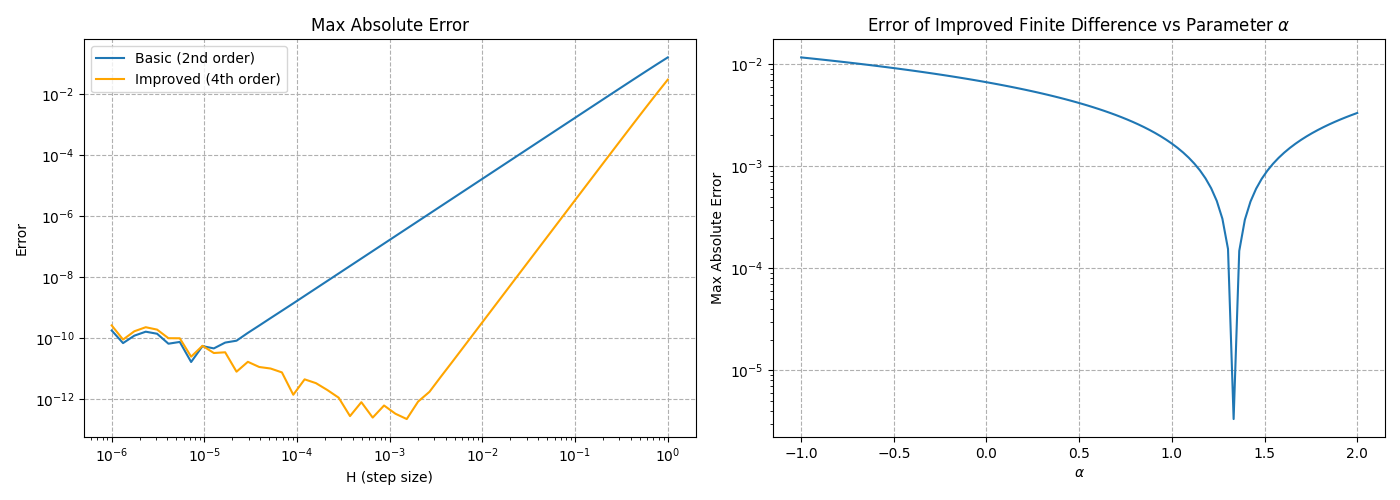
\includegraphics[scale=0.43]{chapters/pm-method/img/finite-difference.png}
    \caption{Left pane: Approximation error for second-order and fourth-order schemes.
        For small values of $H$, round-off errors dominate.
        Right pane: Approximation error vs. $\alpha$ in the improved finite difference scheme ($H = 0.1$).
        Note that the scheme is fourth-order accurate only for $\alpha = 4/3$ (cusp in the graph).}
    \label{fig:finite-diff-accuracy}
\end{figure}

We can alternatively define the finite difference operators in terms of the delta function to get rid of the dependence on the differenced function. (Technically, the resulting quantities are functions rather than operators.)
Consider for example the two-point finite difference in \autoref{eq:two-point-central-diff}.
The definition can be generalized beyond mesh points by letting
\begin{equation*}
    D_j(\phi)(\mathbf{x}) = -\frac{\phi(\mathbf{x} + H \mathbf{e}_j)-\phi (\mathbf{x} - H \mathbf{e}_j)}{2H} = -\int \left[ \frac{\delta(\mathbf{x} + H\mathbf{e}_j - \mathbf{x}') - \delta(\mathbf{x} - H\mathbf{e}_j - \mathbf{x}')}{2H} \right]\phi(\mathbf{x}')d\mathbf{x}',
\end{equation*}
where $\mathbf{e}_j$ is the $j$-th standard basis vector.
This motivates us to define
\begin{equation}\label{eq:two-point-central-diff}
    D_j(\mathbf{x}) = \frac{\delta(\mathbf{x} + H\mathbf{e}_j - \mathbf{x}') - \delta(\mathbf{x} - H\mathbf{e}_j - \mathbf{x}')}{2H}
\end{equation}
and
\begin{equation}\label{eq:four-point-central-diff}
    D_j(\mathbf{x}) = \frac{\delta(\mathbf{x} + H\mathbf{e}_j - \mathbf{x}') - \delta(\mathbf{x} - H\mathbf{e}_j - \mathbf{x}')}{2H} + (1-\alpha)\frac{\delta(\mathbf{x} + 2H\mathbf{e}_j - \mathbf{x}') - \delta(\mathbf{x} - 2H\mathbf{e}_j - \mathbf{x}')}{4H}
\end{equation}
as the two-point as four-point finite difference operators respectively.

If $\phi$ denotes the gravitational potential, then the field $\mathbf{g}$ is approximated at mesh point $\mathbf{x}_\mathbf{p}$ as
\begin{equation*}
    \mathbf{g}(\mathbf{x}_\mathbf{p}) = -\mathbf{D}(\phi)(\mathbf{x}_\mathbf{p}).
\end{equation*}
